\documentclass[notumble,nofoldmark,10pt]{leaflet}

% ============================================
% PACKAGES
% ============================================
\usepackage[utf8]{inputenc}
\usepackage[T1]{fontenc}
\usepackage{graphicx}
\usepackage{enumitem}
\usepackage{hyperref}
\usepackage{xcolor}
\usepackage{tcolorbox}
\usepackage{tikz}
\usepackage{helvet}
\usepackage{microtype}

% Use Helvetica as default sans-serif
\renewcommand{\familydefault}{\sfdefault}

% ============================================
% COLOR SCHEME - Technical Elegant
% ============================================
\definecolor{primaryblue}{HTML}{2563EB}
\definecolor{accentteal}{HTML}{0891B2}
\definecolor{darktext}{HTML}{1F2937}
\definecolor{lightgray}{HTML}{F3F4F6}
\definecolor{medgray}{HTML}{9CA3AF}

% ============================================
% TCOLORBOX STYLES
% ============================================
\tcbuselibrary{skins,breakable}

% Section header style
\newtcolorbox{sectionbox}[1][]{
  enhanced,
  colback=white,
  colframe=white,
  boxrule=0pt,
  left=0pt, right=0pt, top=2pt, bottom=2pt,
  before upper={\textcolor{primaryblue}{\large\bfseries}},
  after upper={\par\vspace{1mm}\textcolor{accentteal}{\rule{\linewidth}{1.5pt}}},
  #1
}

% Highlight box
\newtcolorbox{highlightbox}[1][]{
  enhanced,
  colback=lightgray,
  colframe=primaryblue,
  boxrule=0pt,
  leftrule=3pt,
  arc=0pt,
  left=8pt, right=8pt, top=6pt, bottom=6pt,
  #1
}

% Key insight box
\newtcolorbox{insightbox}[1][]{
  enhanced,
  colback=primaryblue!5,
  colframe=primaryblue,
  boxrule=1pt,
  arc=3pt,
  left=8pt, right=8pt, top=8pt, bottom=8pt,
  #1
}

% ============================================
% PAGE SETUP
% ============================================
\pagestyle{empty}
\setmargins{8mm}{8mm}{8mm}{5mm}

% Custom section command
\newcommand{\bsection}[1]{%
  \vspace{2mm}%
  {\color{primaryblue}\large\bfseries #1}%
  \par\vspace{0.5mm}%
  {\color{accentteal}\rule{0.6\linewidth}{1.5pt}}%
  \par\vspace{2mm}%
}

% Compact itemize
\setlist[itemize]{leftmargin=*, itemsep=1pt, topsep=2pt}
\setlist[enumerate]{leftmargin=*, itemsep=1pt, topsep=2pt}

% ============================================
% DOCUMENT
% ============================================
\begin{document}

% ============================================
% FRONT COVER (Panel 6)
% ============================================

% Background decoration
\begin{tikzpicture}[remember picture, overlay]
  % Top gradient bar
  \fill[primaryblue] (current page.north west) rectangle ([yshift=-15mm]current page.north east);
  % Geometric accent
  \fill[accentteal, opacity=0.8] ([yshift=-15mm, xshift=-20mm]current page.north east) -- ([yshift=-15mm]current page.north east) -- ([yshift=-25mm]current page.north east) -- cycle;
  % Bottom accent line
  \fill[accentteal] (current page.south west) rectangle ([yshift=3mm]current page.south east);
\end{tikzpicture}

\begin{center}
\vspace*{18mm}

{\color{darktext}\LARGE\bfseries Mechanistic Interpretability}

\vspace{1mm}

{\color{darktext}\LARGE\bfseries of Code Correctness in LLMs}

\vspace{4mm}

{\color{accentteal}\large via Sparse Autoencoders}

\vspace{12mm}

% Abstract neural network visual
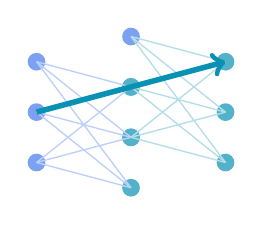
\begin{tikzpicture}[scale=0.8]
  % Nodes
  \foreach \i in {1,2,3} {
    \fill[primaryblue!60] (0, \i*0.8) circle (4pt);
    \fill[accentteal!70] (1.5, \i*0.8-0.4) circle (4pt);
    \fill[primaryblue!60] (1.5, \i*0.8+0.4) circle (4pt);
    \fill[accentteal!70] (3, \i*0.8) circle (4pt);
  }
  % Connections
  \foreach \i in {1,2,3} {
    \foreach \j in {1,2,3} {
      \draw[primaryblue!30, line width=0.5pt] (0, \i*0.8) -- (1.5, \j*0.8-0.4);
      \draw[accentteal!30, line width=0.5pt] (1.5, \i*0.8+0.4) -- (3, \j*0.8);
    }
  }
  % Highlighted path (correctness direction)
  \draw[accentteal, line width=2pt, ->] (0, 1.6) -- (1.5, 2) -- (3, 2.4);
\end{tikzpicture}

\vspace{12mm}

{\color{darktext}\large\bfseries Kriz Royce Tahimic}

\vspace{2mm}

{\color{medgray}\small Adviser: Dr. Charibeth K. Cheng}

\vspace{8mm}

{\color{darktext}\small College of Computer Studies}\\
{\color{primaryblue}\small\bfseries De La Salle University}

\vspace{5mm}

{\color{medgray}\footnotesize Academic Year 2024--2025}

\end{center}

\newpage

% ============================================
% INSIDE LEFT (Panel 1) - Context & Problem
% ============================================

% Top decoration
\begin{tikzpicture}[remember picture, overlay]
  \fill[primaryblue] (current page.north west) rectangle ([yshift=-4mm]current page.north east);
\end{tikzpicture}

\vspace{2mm}

\bsection{Context}

{\small
AI-assisted coding has reached critical mass:
\begin{itemize}
  \item \textbf{30\%} of GitHub Copilot suggestions enter production code
  \item Projected \textbf{\$1.5 trillion} GDP impact by 2030
  \item LLMs increasingly deployed in critical systems
\end{itemize}
}

\vspace{2mm}

\bsection{The Problem}

\begin{highlightbox}
{\small\color{darktext}
We lack \textbf{mechanistic understanding} of WHEN and WHY models produce correct code.
}
\end{highlightbox}

{\small
\begin{itemize}
  \item Models fail in bug-prone contexts (12.27\% accuracy)
  \item 44\% of LLM bugs mirror historical training bugs
  \item Critical for: healthcare, banking, military
\end{itemize}
}

\vspace{2mm}

\bsection{The Challenge}

{\small
Neural networks are hard to interpret:
\begin{itemize}
  \item \textbf{Polysemantic neurons}: One neuron responds to multiple unrelated concepts
\end{itemize}
}

\vspace{1mm}

\begin{center}
\includegraphics[width=0.95\linewidth]{figures/polysemantic neuron.png}
\end{center}

{\scriptsize\color{medgray}\centering A single neuron activates for unrelated concepts (cat, car, citation)\par}

\newpage

% ============================================
% INSIDE CENTER (Panel 2) - Approach
% ============================================

\begin{tikzpicture}[remember picture, overlay]
  \fill[primaryblue] (current page.north west) rectangle ([yshift=-4mm]current page.north east);
\end{tikzpicture}

\vspace{2mm}

\bsection{Why Interpretation is Hard}

{\small
\textbf{Superposition}: Networks compress more features than dimensions, entangling representations.
}

\vspace{1mm}

\begin{center}
\includegraphics[width=0.85\linewidth]{figures/superposition.png}
\end{center}

{\scriptsize\color{medgray}\centering Features compressed into overlapping directions\par}

\vspace{3mm}

\bsection{Our Approach}

{\small
\textbf{Sparse Autoencoders (SAEs)} decompose entangled representations into interpretable directions.
}

\vspace{2mm}

\begin{highlightbox}
{\small
\textbf{Key Idea}: If code correctness is represented as a \emph{direction} in the model's latent space, we can:
\begin{enumerate}[itemsep=1pt]
  \item \textbf{Detect} it (prediction)
  \item \textbf{Manipulate} it (steering)
  \item \textbf{Validate} it (causal analysis)
\end{enumerate}
}
\end{highlightbox}

\vspace{3mm}

{\small
\textbf{Technical Setup}:
\begin{itemize}
  \item \textbf{Model}: Gemma-2 2B (base \& instruction-tuned)
  \item \textbf{SAE}: GemmaScope pre-trained (16K features)
  \item \textbf{Dataset}: MBPP (1,000 Python problems)
  \item \textbf{Analysis}: Residual stream at layer 20
\end{itemize}
}

\newpage

% ============================================
% INSIDE RIGHT (Panel 3) - Key Insight
% ============================================

\begin{tikzpicture}[remember picture, overlay]
  \fill[primaryblue] (current page.north west) rectangle ([yshift=-4mm]current page.north east);
\end{tikzpicture}

\vspace{2mm}

\bsection{Key Discovery}

\begin{insightbox}
{\color{darktext}
\textbf{Code correctness directions EXIST} in LLM representations---and they are \textbf{actionable}.
}
\end{insightbox}

\vspace{3mm}

{\small
\textbf{1. Predict Errors Before Generation}

The \textbf{incorrect-predicting direction} detects errors with high accuracy:
}

\vspace{1mm}

\begin{center}
\includegraphics[width=0.95\linewidth]{figures/incorrect-predicting.png}
\end{center}

{\scriptsize\color{medgray}\centering F1: 0.821 for error detection---can serve as ``error alarm''\par}

\vspace{3mm}

{\small
\textbf{2. Steer Toward Correctness}

The \textbf{correct-steering direction} can fix errors (4.04\% of incorrect code fixed).

\vspace{2mm}

\textbf{3. Asymmetric Finding}

\begin{itemize}
  \item Found: \textbf{incorrect-predicting} + \textbf{correct-steering}
  \item Did NOT find: correct-predicting or incorrect-steering
  \item \emph{Models detect ``wrongness'' differently than they encode ``correctness''}
\end{itemize}
}

\newpage

% ============================================
% BACK CENTER (Panel 4) - Mechanistic Findings
% ============================================

\begin{tikzpicture}[remember picture, overlay]
  \fill[accentteal] (current page.north west) rectangle ([yshift=-4mm]current page.north east);
\end{tikzpicture}

\vspace{2mm}

\bsection{Mechanistic Evidence}

{\small
Multiple analyses validate our findings:

\vspace{2mm}

\textbf{Prediction Analysis}
\begin{itemize}
  \item Incorrect-predicting: \textbf{F1 = 0.821}
  \item Correct-predicting: F1 = 0.504 (weak)
\end{itemize}

\vspace{1mm}

\textbf{Steering Interventions}
\begin{itemize}
  \item Correct-steering fixes 4.04\% of errors
  \item Trade-off: affects 14.66\% correct code
\end{itemize}

\vspace{1mm}

\textbf{Attention Analysis}
}

\begin{center}
\includegraphics[width=0.95\linewidth]{figures/attention_delta_plots.png}
\end{center}

{\scriptsize\color{medgray}\centering Test cases matter MORE than problem descriptions\par}

\vspace{2mm}

{\small
\textbf{Necessity (Orthogonalization)}
\begin{itemize}
  \item Removing correct directions: 83.62\% code corruption
  \item Control removal: only 18.97\% corruption
\end{itemize}

\vspace{1mm}

\textbf{Persistence Across Fine-tuning}
\begin{itemize}
  \item Base $\rightarrow$ Instruction-tuned: F1 0.821 $\rightarrow$ 0.772
  \item Mechanisms learned in pre-training persist
\end{itemize}
}

\newpage

% ============================================
% BACK RIGHT (Panel 5) - Significance & Contact
% ============================================

\begin{tikzpicture}[remember picture, overlay]
  \fill[accentteal] (current page.north west) rectangle ([yshift=-4mm]current page.north east);
\end{tikzpicture}

\vspace{2mm}

\bsection{Significance}

\begin{highlightbox}
{\small
\textbf{First application} of Sparse Autoencoders to study code correctness mechanisms in LLMs.
}
\end{highlightbox}

\vspace{2mm}

{\small
\textbf{Practical Applications}:
\begin{enumerate}[itemsep=2pt]
  \item \textbf{Prompting strategies}: Prioritize test examples over problem descriptions
  \item \textbf{Error alarms}: Predictor directions flag code for developer review
  \item \textbf{Selective steering}: Intervene only when errors anticipated
\end{enumerate}

\vspace{2mm}

\textbf{Safety Implications}: Contributes to safer AI deployment in healthcare, finance, and critical infrastructure.
}

\vspace{3mm}

\bsection{Key References}

{\scriptsize
\begin{itemize}[itemsep=0pt]
  \item Bricken et al. (2023) --- Towards Monosemanticity
  \item Templeton et al. (2024) --- Scaling Monosemanticity
  \item Lieberum et al. (2024) --- GemmaScope
  \item Ferrando et al. (2024) --- Entity Recognition via SAEs
\end{itemize}
}

\vspace{3mm}

\bsection{Contact}

{\small
\textbf{Proponent}:\\
Kriz Royce Tahimic\\
{\color{primaryblue}\small kriz\_tahimic@dlsu.edu.ph}

\vspace{2mm}

\textbf{Adviser}:\\
Dr. Charibeth K. Cheng\\
{\color{primaryblue}\small charibeth.cheng@dlsu.edu.ph}
}

\vspace{3mm}

\begin{center}
{\small\bfseries College of Computer Studies}\\
{\small De La Salle University}\\
{\small Manila, Philippines}\\[2mm]
{\scriptsize\color{medgray} BS Computer Science --- Software Technology}
\end{center}

\end{document}
